\documentclass[12pt,reqno]{amsart}
\usepackage{/Users/johnmyers/tex/handout,/Users/johnmyers/tex/customcommands,polynom}
\usepackage{caption}

\hdr{MAT 240}{18 Integrals of functions of two variables}

\begin{document}

\bigskip

\prob The contour diagram of a function $f$ is shown below. Estimate $\int_R f \ dA$ if $R$ is the rectangular region with $0 \leq x \leq 30$ and $0 \leq y \leq 15$.


\includegraphics[scale=1.25]{pic1.pdf}

\vfill
\prob The table below gives the values of $f(x,y)$, the number of milligrams of mosquito larvae per square meter in a swamp. If $x$ and $y$ are in meters and $R$ is the rectangle with $0 \leq x \leq 8$ and $0 \leq y \leq 6$, estimate $\int_R f \ dA$. Give units and interpret your answer.

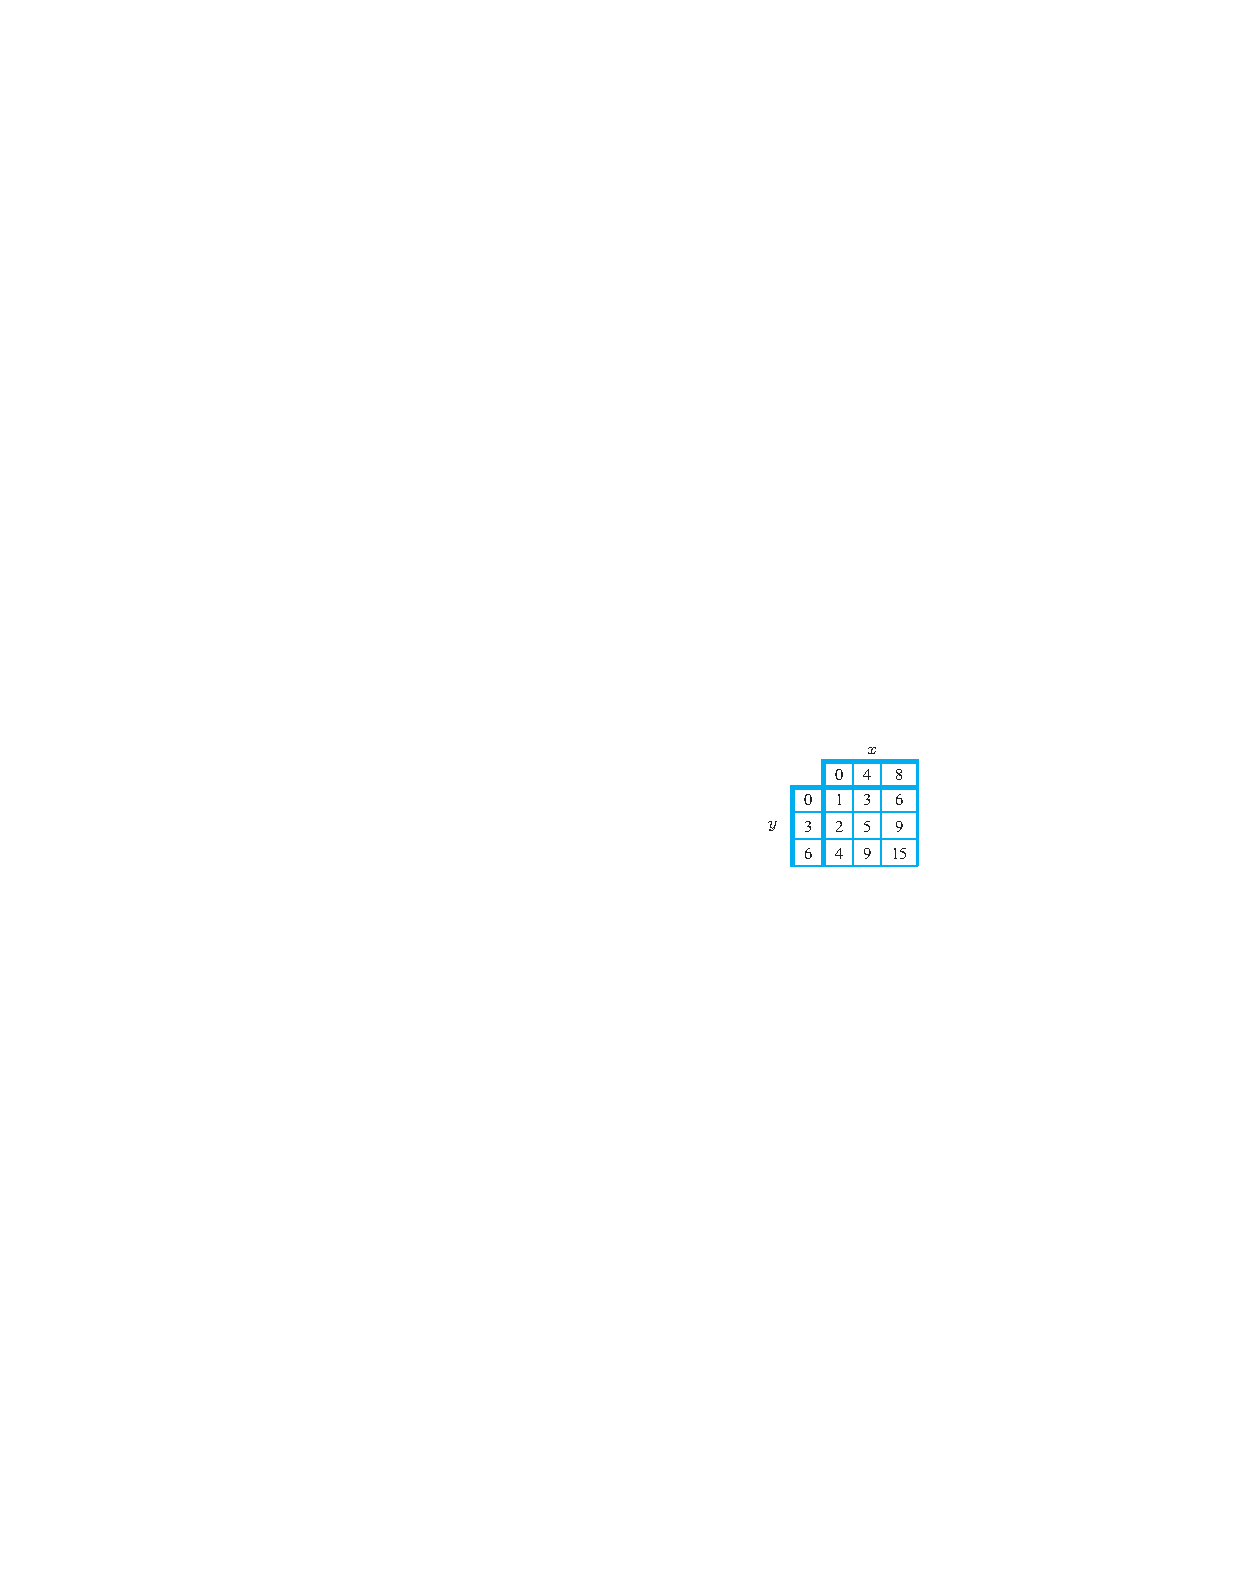
\includegraphics[scale=1.25]{pic2.pdf}

\vfill
\prob The figure below shows a contour plot of population density, people per square kilometer, in a rectangle of land 3 km by 2 km. Estimate the population in this region.

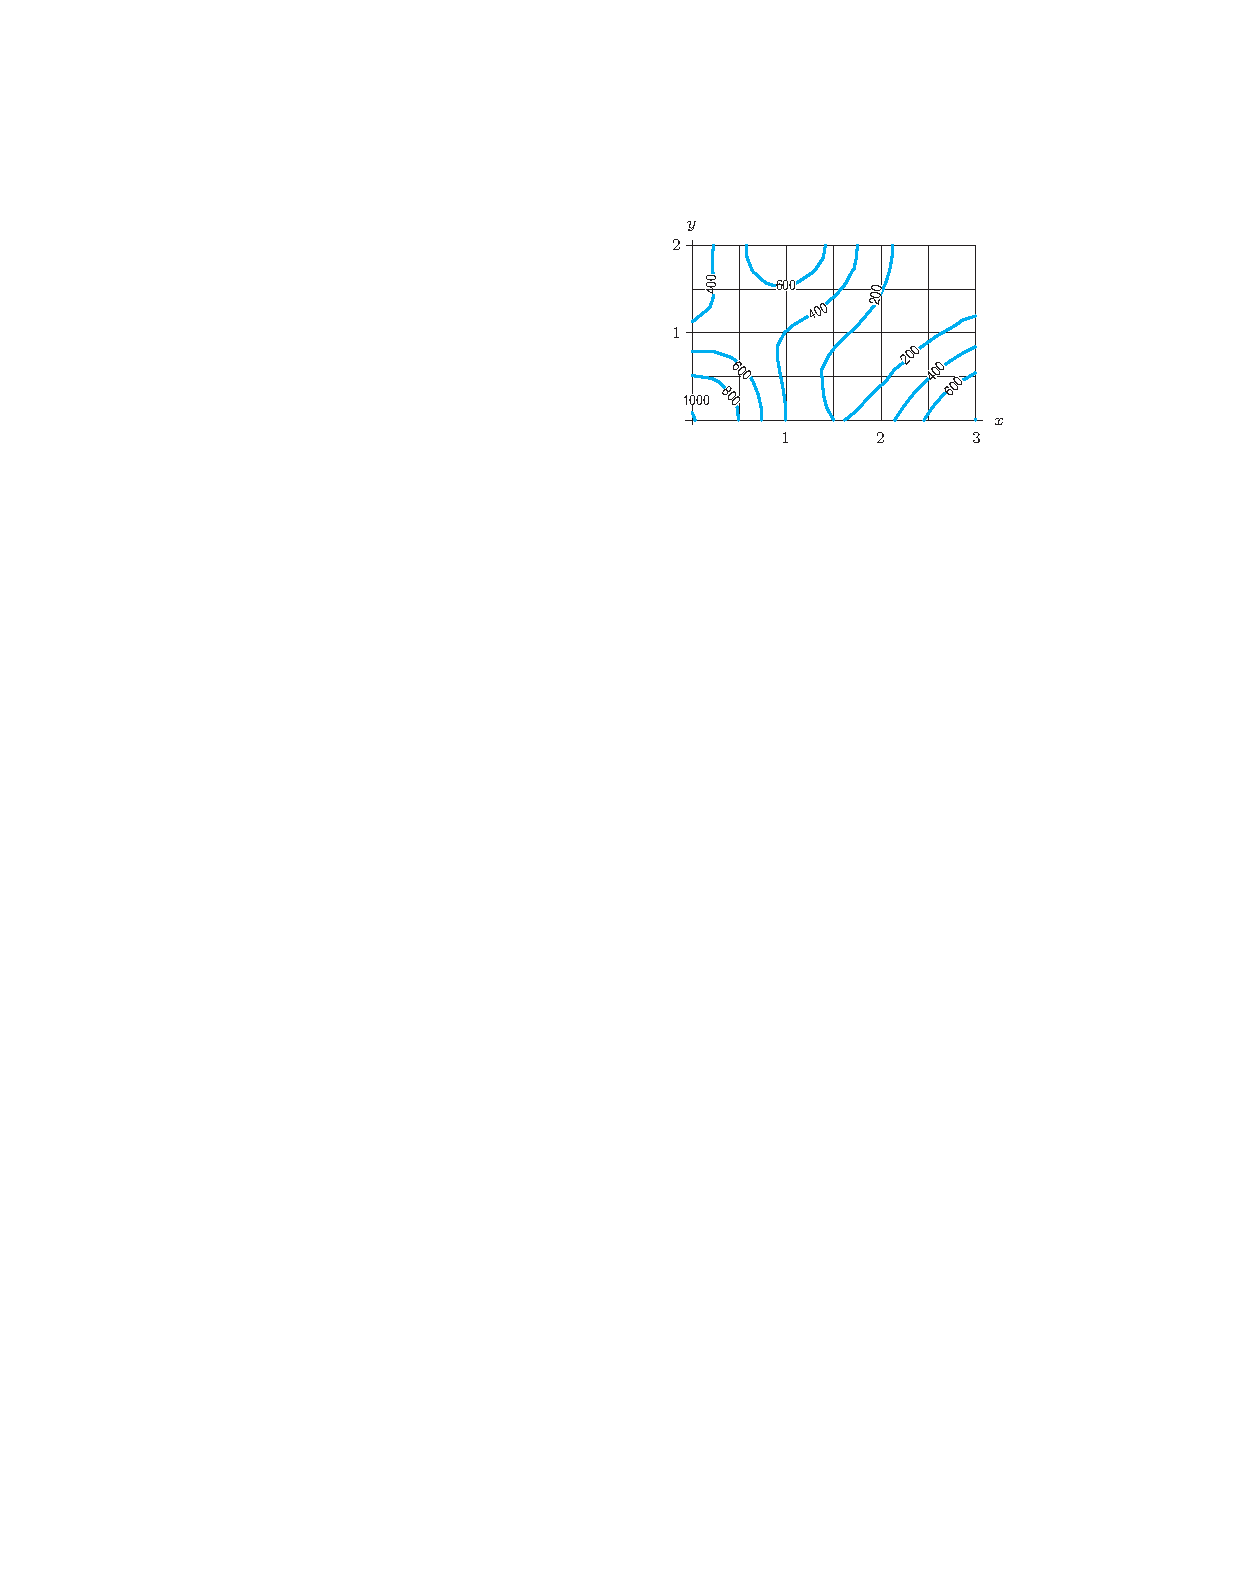
\includegraphics[scale=1]{3.pdf}

\vfill
\newpage
\prob If $R$ is the rectangle $[0,2] \times [0,4]$, then evaluate
	\[\int_R 2x \ dA.
	\]



\end{document}